\scanpage{97}
Soit $u'$ le composé $\deleted{\unsure{u'_{j,n}}}\quad B\quad E_{k,n}\qquad E'_{j,n}\ {\vphantom{E'}}^{u'_{j,\unsure{n|h}}}\ D'$, où la première flèche est l'hom de transition, alors $u'$ est le relèvement cherché.

Mettre le corollaire 2.2. sous forme de l'équivalence de trois conditions (i) $B$ form simple (ii) Condition $1^\circ$ et $2^\circ$ (iii) $\widehat B$ est isomorphe comme alg top à $\widehat {B'}$, où $B'$ est l'algèbre symétrique d'un $C$-module projectif, munie de \unsure{sa|la} topologie définie par son idéal d'augmentation. La forme (iii) est en effet parfois commode, et est obtenue directement dans la démonstration.
\margin{\figure{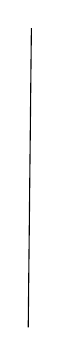
\begin{tikzpicture}\draw (0,0)--(-.04,-3.8);\end{tikzpicture}}}
\margin{\unsure{(i bis)} Pour tout hom de $B$ dans \deleted{une \unsure{$A$-algèbre, quotient} $\unsure{C'|B'}\ D'/J$}, $B'$ \deleted{\unsure{discrète et}} considérée comme quotient d'un \unsure{$\Lambda_D$|$A_D$}. \unsure{polynômiale tronquée}, \deleted{\unsure{on peut relever}} \unsure{on a un} \deleted{$C[t]$} $B'_{\unsure{(i)|i}}$ de $B'_0=C$, \unsure{on peut relever}}
\margin{$\unsure{B'I/I^2}\ \longleftrightarrow$\quad de type fini}

Dans la suite du paragraphe Cohen, 3.4. devient un corollaire immédiat de 3.3. grâce à 2.2. D'ailleurs 3.3. admet toute une kyrielle de corollaires qui dans ma rédaction étaient dans un ordre assez chaotique, je suggère \deleted{\unsure{le}} l'ordre suivant:

$1^\circ$ Existence d'un corps de représentants dans un anneau \inserted{local noeth} complet, quand l'extension résiduelle est séparable. (Cf 3.5.)

$2^\circ$ (oublié dans ma rédaction). Soit $A$ anneau local noeth complet. Les conditions suivantes sont équivalentes: (i) $A$ contient un corps

(ii) Si $\operatorname{car}k(A)=p\quad0$, alors $pA=0$ (iii) $A$ est isomorphe à un anneau quotient d'un anneau $k\ T_1,\ldots,T_n$ sur un corps $k$. (iv) (Si $A$ est intègre de corps des fractions $K$) $k(A)$ et $K$ ont même caractéristique. On peut se borner à donner (iv) à titre de commentaire (c'est une autre façon d'énoncer (ii) simplement), pour \deleted{\unsure{rappeler}} rappeler l'ancienne terminologie ``cas d'égale caractéristique''. Je suggère que nous ne suivions pas cette terminologie, car il est aussi court de dire ``$A$ contient un corps'', et la terminologie ``égale car'' est fort ambigue pour des anneaux non intègres, par exemple artiniens.
\margin{96}
